\documentclass{article}
\usepackage[utf8]{inputenx}
\usepackage[margin=1in]{geometry}
\usepackage{amsmath, textcomp, amssymb, caption, subcaption}

\renewcommand{\Re}{\mathrm{Re}}
\renewcommand{\Im}{\mathrm{Im}}

\usepackage{tikz, tkz-euclide, pgfplots}
\usetikzlibrary{shapes, patterns, positioning, shapes.gates.logic.US}

\tikzset{
	odot/.style={
		circle,
		inner sep=0pt,
		node contents={$\odot$},
		scale=2
	},
	otimes/.style={
		circle,
		inner sep=0pt,
		node contents={$\otimes$},
		scale=2
	},
	circ/.style={
		circle,
		draw,
		minimum size=5mm,
		inner sep=0
	}
}

\pgfplotsset{compat=newest}
\pgfplotsset{soldot/.style={color=green,only marks,mark=*}}
\pgfplotsset{holdot/.style={color=black,only marks,mark=*}}

\newcommand{\ihat}{\hat{\imath}}
\newcommand{\jhat}{\hat{\jmath}}
\newcommand{\khat}{\hat{k}}

\begin{document}
	\begin{figure}
		\centering 
		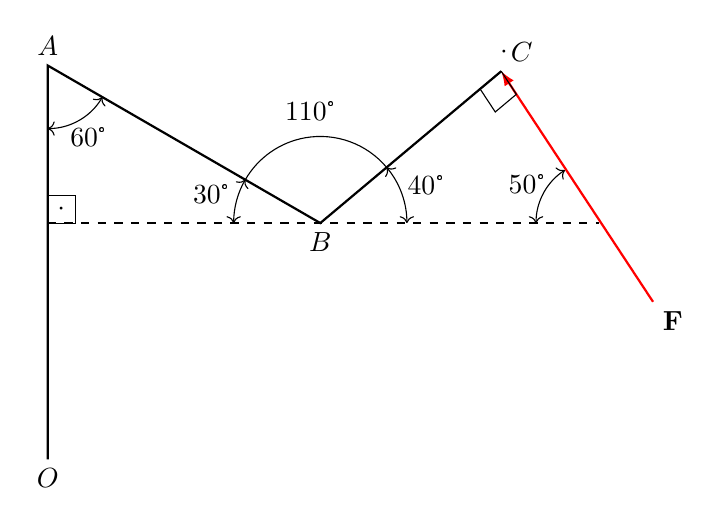
\begin{tikzpicture}
		\coordinate[label=below:$O$] (O) at (0,0);
		\coordinate[label=above:$A$] (A) at (0,5);
		\coordinate[label=below:$B$] (B) at (3.46,3);
		\coordinate[label=above right:$C$] (C) at (5.758,4.928);
		\coordinate (X) at (0,3);
		\coordinate (Y) at (7,3);
		\coordinate (Z) at (0,3);
		\coordinate[label=below right:$\mathbf{F}$] (F) at (7.686,2);
		
		\draw[thick] (O)--(A)--(B)--(C);
		\draw[dashed, thick] (X)--(Y);
		\draw[thick, -latex, red] (F)--(C);
		
		\draw pic["30\textdegree", draw=black, <->, angle eccentricity=1.3, angle radius=1.1cm]{angle=A--B--X}; 
		
		
		\draw pic["40\textdegree", draw=black, <->, angle eccentricity=1.3, angle radius=1.1cm]{angle=Y--B--C}; 
		
		\draw pic["50\textdegree", draw=black, <->, angle eccentricity=1.3, angle radius=0.8cm]{angle=C--Y--B};
		
		\draw pic["60\textdegree", draw=black, <->, angle eccentricity=1.3, angle radius=0.8cm]{angle=O--A--B};
		
		\draw pic["110\textdegree", draw=black, angle eccentricity=1.3, angle radius=1.1cm]{angle=C--B--A}; 
		
		\tkzMarkRightAngle[size=0.35](B,Z,A);
		\tkzLabelAngle[dist=.24](B,Z,A){$\cdot$};
		
		\tkzMarkRightAngle[size=0.35](F,C,B);
		\tkzLabelAngle[dist=.24](F,C,B){$\cdot$};
		\end{tikzpicture}
	\end{figure}

	\begin{figure}
		\centering
		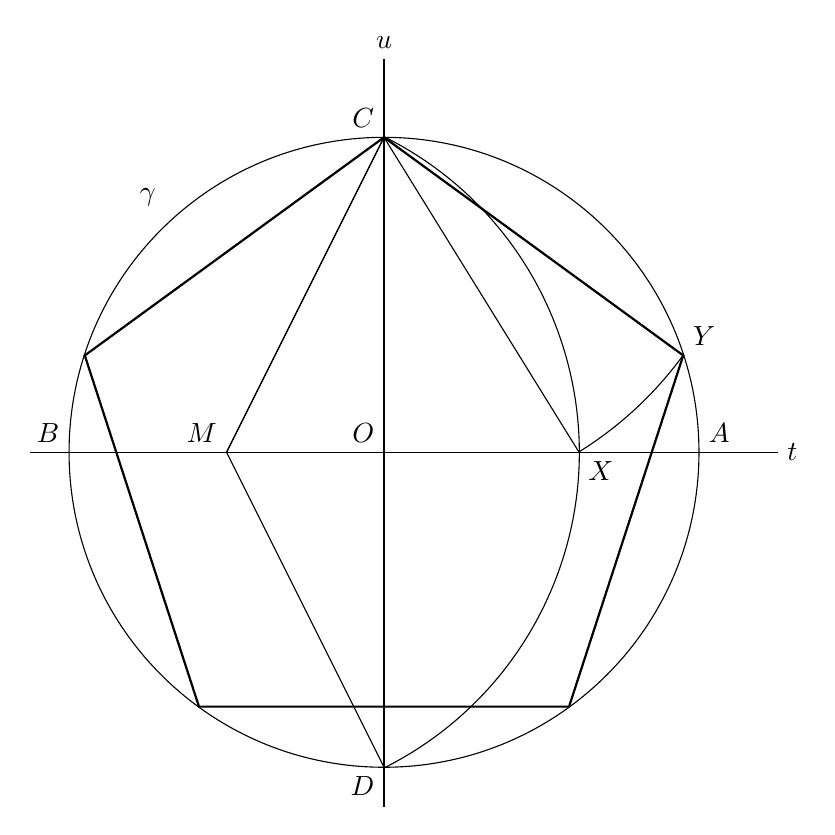
\begin{tikzpicture}
		\draw (0, 0) circle [radius=4];
		\coordinate[label=above left:$O$] (O) at (0,0);
		\coordinate[label=$\gamma$] (g) at (-3,3);
		\draw (-4.5, 0) -- (5, 0);
		\coordinate[label=right:$t$] (t) at (5,0);
		\coordinate[label=above right:$A$] (A) at (4,0);
		\coordinate[label=above left:$B$] (B) at (-4,0);
		\coordinate[label=above left:$M$] (M) at (-2,0);
		\draw (0,-4.5) -- (0,5);
		\coordinate[label=above:$u$] (u) at (0,5);
		\coordinate[label=above left:$C$] (C) at (0,4);
		\coordinate[label=below left:$D$] (D) at (0,-4);
		\draw (M) -- (C);
		\draw (M) -- (D);
		\draw (M) -- +(63.43:4.48) arc (63.43:-63.43:4.48);
		\coordinate[label=below right:$X$] (X) at (2.47,0);
		\draw (C) -- +(-58.23:4.7) arc (-58.23:-36:4.7);
		
		\coordinate[label=above right:$Y$] (Y) at (3.8,1.23);
		\coordinate (V) at (-3.8,1.23);
		\coordinate (W) at (-2.35,-3.23);
		\coordinate (Z) at (2.35,-3.23);
		
		\draw[thick] (Y) -- (C) -- (V) -- (W) -- (Z) -- cycle;		
		\end{tikzpicture}
	\end{figure}

	\begin{figure}[h!]
		\centering
		\begin{tikzpicture}
		% A, B, C e corda
		\coordinate[label=above right: \large{$A$}] (A) at (0,2);
		\coordinate[label=above: \large{$C$}] (C) at (2,-1);
		\coordinate[label=above left: \large{$B$}] (B) at (5,4);
		\draw plot [smooth, ultra thick] coordinates {(A) (C) (B)};	
		
		% TA
		\coordinate (P) at (-1,2);
		\coordinate (Q) at (1,-0.5);
		\coordinate (R) at (1,2);
		\coordinate (S) at (-1,4.5);
		
		\draw[dashed] (A)--(Q);
		\draw[dashed] (R)--(P);
		\draw[-latex, very thick] (A)--(S) node [at end, above left]{\large{$\mathbf{T_A}$}}; 	
		
		\draw pic["\large{$\theta$}", draw=black, angle eccentricity=1.3, angle radius=0.6cm]{angle=S--A--P};
		\draw pic["\large{$\theta$}", draw=black, angle eccentricity=1.3, angle radius=0.6cm]{angle=Q--A--R};
		
		% TB
		\coordinate (X) at (4,4);
		\coordinate (Y) at (6,4);
		\coordinate (Z) at (6,6);
		\coordinate (W) at (4,1.8);
		
		\draw[dashed] (X)--(Y);
		\draw[-latex, very thick] (B)--(Z) node [at end, above right]{\large{$\mathbf{T_B}$}};
		\draw[dashed] (B)--(W);
		
		\draw pic["\large{$\alpha$}", draw=black, angle eccentricity=1.4, angle radius=0.6cm]{angle=Y--B--Z};
		\draw pic["\large{$\alpha$}", draw=black, angle eccentricity=1.4, angle radius=0.6cm]{angle=X--B--W};
		
		% T
		\draw[-latex, very thick] (C)--(4,-1) node [at end, right]{\large{$\mathbf{T}$}};
		
		% P
		\draw[very thick, -latex] (C)--(2,-4) node [midway, right]{\large{$\mathbf{P}$}};
		\end{tikzpicture}
	\end{figure}

	\begin{figure}[h!]\centering
		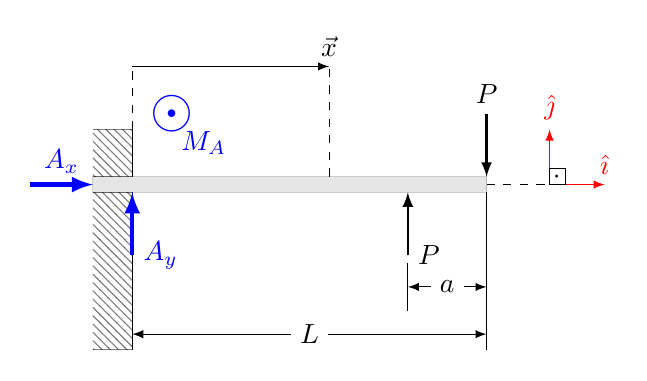
\begin{tikzpicture}
		% viga
		\draw[fill=gray, opacity=0.2] (0,0)--(0,0.2)--(5,0.2)--(5,0)--cycle;
		
		% engaste
		\draw (0.5,-2)--(0.5,0);
		\draw (0.5,0.2)--(0.5,0.8);
		\draw[pattern=north west lines, opacity=0.5] (0,0)--(0.5,0)--(0.5,-2)--(0,-2);
		\draw[pattern=north west lines, opacity=0.5] (0,0.2)--(0.5,0.2)--(0.5,0.8)--(0,0.8);
		
		% P's
		\draw[-latex, thick] (5,1)--(5,0.2) 
		node [at start, above] {$P$};
		\draw[-latex, thick] (4,-0.8)--(4,0) 
		node [at start, right] {$P$};
		
		% comprimentos
		\draw (5,0)--(5,-2);
		\draw (4,-0.9)--(4,-1.5);
		% a
		\draw[latex-latex] (4,-1.2)--(5,-1.2)
		node [midway, fill=white] {$a$};
		% L
		\draw[latex-latex] (0.5,-1.8)--(5,-1.8)
		node [midway, fill=white] {$L$};
		
		% esforçoes
		% Ay
		\draw[-latex, blue, ultra thick] (0.5,-0.8)--(0.5,0)
		node [at start, right] {$A_y$};
		% Ax
		\draw[-latex, blue, ultra thick] (-0.8,0.1)--(0,0.1)
		node [midway, above] {$A_x$};
		% M_A
		\node[odot, blue, at={(1,1)}];	
		\draw (1,0.9)--(1,0.9) node [blue, below right] {$M_A$};
		
		% vetor x
		\draw[dashed] (0.5,0.8)--(0.5,1.6);
		\draw[dashed] (3,0.2)--(3,1.6);
		\draw[-latex] (0.5,1.6)--(3,1.6)
		node [at end, above] {$\vec{x}$};
		
		% direções i, j
		\coordinate (O) at (5.8,0.1);
		\coordinate (i) at (6.5,0.1);
		\coordinate (j) at (5.8,0.8);
		
		\draw[dashed] (5,0.1)--(5.8,0.1);
		% i
		\draw[-latex, red] (O)--(i)
		node [at end, above] {$\ihat$};
		% j
		\draw[-latex, red] (O)--(j)
		node [at end, above] {$\jhat$};
		
		\tkzMarkRightAngle[size=0.2](i,O,j);
		\tkzLabelAngle[dist=.13](i,O,j){$\cdot$};
		\end{tikzpicture}
	\end{figure}

	\begin{figure}[h!]\centering
		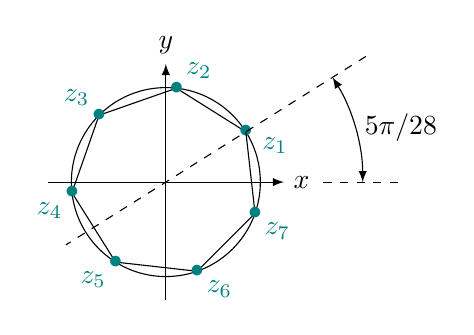
\begin{tikzpicture}
		\draw [-latex] (-1.5, 0) -- (1.5, 0) node [at end, right] {$x$};
		\draw [-latex] (0, -1.5, 0) -- (0, 1.5) node [at end, above] {$y$};
		
		\draw (0,0) circle (1.2cm);
		\foreach \x in {0, 51.428, ..., 308.568} {
			\draw (32.142+\x:1.2) -- (32.142+\x+51.428:1.2);
			\node [teal] at (\x+32.142:1.2) {$\bullet$};
		}
		\node [at={(32.142:1.3)}, teal, below right] {$z_1$};
		\node [at={(32.142 + 51.428:1.2)}, teal, above right] {$z_2$};
		\node [at={(32.142 + 2*51.428:1.2)}, teal, above left] {$z_3$};
		\node [at={(32.142 + 3*51.428:1.2)}, teal, below left] {$z_4$};
		\node [at={(32.142 + 4*51.428:1.2)}, teal, below left] {$z_5$};
		\node [at={(32.142 + 5*51.428:1.2)}, teal, below right] {$z_6$};
		\node [at={(32.142 + 6*51.428:1.2)}, teal, below right] {$z_7$};
		
		\draw [dashed] (32.142:3) -- (180+32.142:1.5);
		\draw [dashed] (2,0)--(3,0);
		\draw [latex-latex] (0:2.5) arc (0:32.142:2.5) node [midway, right] {$5\pi/28$};
		\end{tikzpicture}
	\end{figure}

	\begin{figure}[h!]\centering
		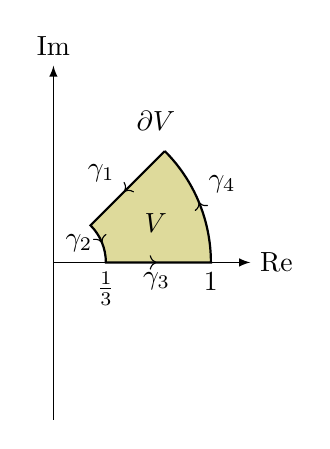
\begin{tikzpicture}
		\draw [fill=olive!30, thick]
		(45:2cm)--(45:0.666cm) 
		arc (45:0:0.666cm)--(0:2cm) 
		arc	(0:45:2cm)
		;
		\draw[-latex] (0,0)--(2.5,0) 
		node [at end, right] {$\Re$}
		node [at={(2,0)}, below] {$1$}
		node [at={(2/3,0)}, below] {$\frac{1}{3}$};
		
		\draw[-latex] (0,-2)--(0,2.5)
		node [at end, above] {$\Im$};	
		
		\draw[->] (1,1)--(0.9,0.9)
		node [at end, above left] {$\gamma_1$};
		
		\draw[->] (30:2/3) arc (30:22:2/3)
		node [at end, left] {$\gamma_2$};
		
		\draw[->] (1.3,0)--(1.31,0)
		node [at end, below] {$\gamma_3$};	
		
		\draw[->] (22:2) arc (22:22.5:2)
		node [at end, above right] {$\gamma_4$};
		
		\node at (1.3, 0.5) {$V$};
		\node at (1.3, 1.8) {$\partial V$};
		\end{tikzpicture}
	\end{figure}

	\begin{figure}[h!]\centering
		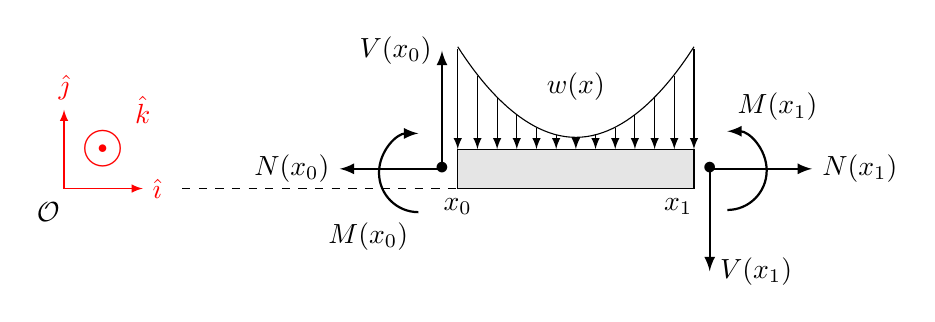
\begin{tikzpicture}
		%% i, j, k, A
		\draw [-latex, red] (-5, 0) -- (-4, 0) node [at end, right] {$\ihat$};
		\draw [-latex, red] (-5, 0) -- (-5, 1) node [at end, above] {$\jhat$};
		\node [odot, red, at={(-4.5, 0.5)}];
		\node [at={(-4, 1)}, red] {$\khat$}; 
		\node at (-5.2, -0.3) {$\mathcal{O}$};
		
		%% Comprimento de viga
		\draw [dashed] (-3.5, 0) -- (1,0);
		\draw [fill=gray!20] (0,0) -- (3,0) -- (3,1/2) -- (0,1/2) -- cycle
		node [at={(0,0)}, below] {$x_0$}
		node [at={(2.8,0)}, below] {$x_1$};		
		
		%% q, A_y, N, V, M, 
		%\draw [very thick, purple] (10,0) parabola bend (10.75,1) (12,-2);
		\draw (0,1.8) parabola bend (1.5, 0.65) (3, 1.8) node [at={(1.5,1)}, above] {$w(x)$};
		\foreach \i in {0, 0.25, ..., 3} {
			\draw [-latex] (\i, 0.5*\i*\i-1.5*\i+3.55*0.5) -- (\i,1/2);
		}
		
		\draw [thick, latex-] (-0.5, 0.7) arc (90:270:0.5) node [at end, below left]{$M(x_0)$};
		\draw [-latex, thick] (-0.2, 1/4) -- (-1.5, 1/4) node [at end, left] {$N(x_0)$}
		node [at start] {$\bullet$};
		\draw [-latex, thick] (-0.2, 1/4) -- (-0.2, 1.75) node [at end, left] {$V(x_0)$};
		
		\draw [thick, latex-] (12:3.5) arc (90:-90:0.5) node [at start, above right] {$M(x_1)$};
		\draw [-latex, thick] (3.2, 1/4) -- (4.5, 1/4) node [at end, right] {$N(x_1)$}
		node [at start] {$\bullet$};
		\draw [-latex, thick] (3.2, 1/4) -- (3.2, -1.05) node [at end, right] {$V(x_1)$};
		\end{tikzpicture}
	\end{figure}

	\begin{figure}[h!]\centering
		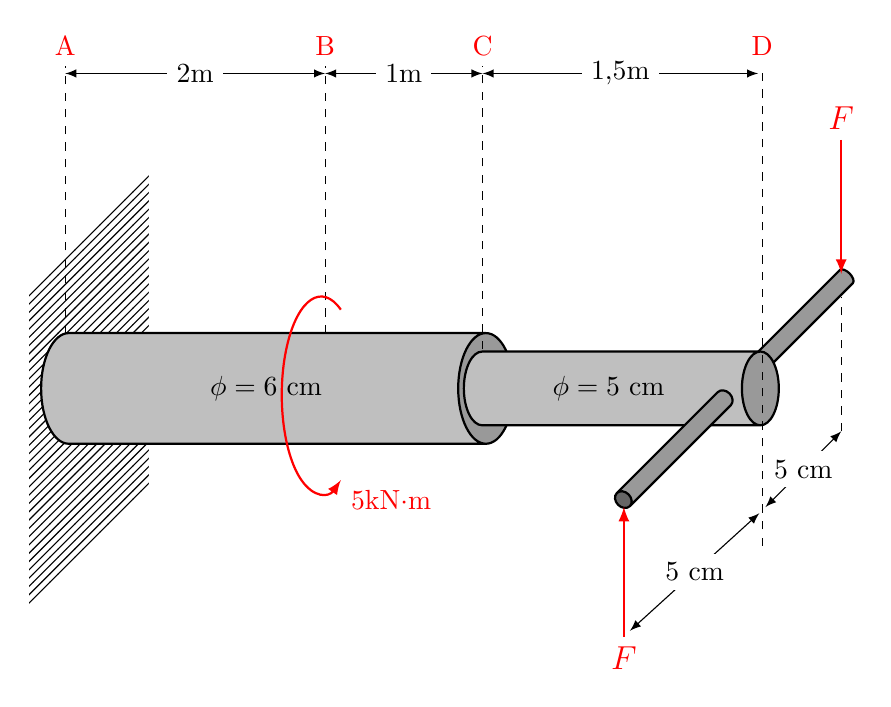
\begin{tikzpicture} [> = latex]
		\draw [color=white, pattern = north east lines]
		(-2,-2,2) -- (-2,-2,-2) -- (-2,2,-2) -- (-2,2,2) -- cycle;
		
		\node[thick, cylinder, draw, shape aspect=0.5,  
		cylinder uses custom fill, cylinder end fill=black!40, minimum height=1cm,
		cylinder body fill=black!25, scale=6]{};
		
		\begin{scope}[shift={(7,0.8)}]	
		\node[thick, cylinder, draw, shape aspect=0.5,  
		cylinder uses custom fill, cylinder end fill=black!60, minimum height=2cm,
		cylinder body fill=black!40, scale=1, rotate=225]{};	
		\end{scope}
		
		\begin{scope}[shift={(4.5,0)}]	
		\node[thick, cylinder, draw, shape aspect=0.5,  
		cylinder uses custom fill, cylinder end fill=black!40, minimum height=1cm,
		cylinder body fill=black!25, scale=4]{};	
		\end{scope}
		
		\begin{scope}[shift={(5.5,-0.7)}]	
		\node[thick, cylinder, draw, shape aspect=0.8,  
		cylinder uses custom fill, cylinder end fill=black!60, minimum height=2cm,
		cylinder body fill=black!40, scale=1, rotate=225]{};
		\end{scope}
		
		\draw [dashed] 
		(-2.3, 0.7,0) -- (-2.3, 4.1,0) node [at end, above, red] {A}
		(1, 0.7,0) -- (1,4.1,0) 	   node [at end, above, red] {B}
		(3, 0.5,0) -- (3, 4.1,0) 	   node [at end, above, red] {C}
		(6.55, -2,0) -- (6.55, 4.1,0)  node [at end, above, red] {D}
		(6.4, -1.7, -3) -- (6.4, 0, -3);
		
		\draw [thick, ->, red] (6.4, 2, -3) -- (6.4, 0.3, -3) 
		node [at start, above]  {\large{$F$}};
		
		\draw [thick, ->, red] (5.95,-2, 3) -- (5.95,-0.35,3) 
		node [at start, below] {\large{$F$}};
		
		\draw [<->] (6.4, -1.7, -0.3) -- (5.95, -2, 2.8) node [midway, fill=white] {5 cm};
		\draw [<->] (6.4, -1.7, -3) -- (6.4, -1.7, -0.5) node [midway, fill=white] {5 cm};
		
		\draw [<->] (-2.3, 4,0) -- (1,4,0) node [midway, fill=white] {2m};
		\draw [<->] (3, 4,0) -- (1,4,0) node [midway, fill=white] {1m};
		\draw [<->] (3, 4,0) -- (6.5,4,0) node [midway, fill=white] {1,5m};
		
		\node at (0.25,0,0) {$\phi=6$ cm};
		\node at (4.6,0,0) {$\phi=5$ cm};
		
		\draw [thick, red, ->] (1.2,1) arc (60:300: 0.5 and 1.25) 
		node [at end, below right] {5kN$\cdot$m};
		\end{tikzpicture}
	\end{figure}

	\begin{figure}[h!]\centering
		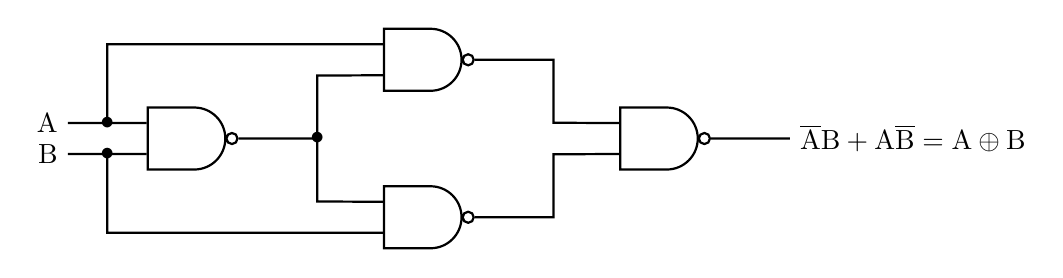
\begin{tikzpicture}[
		thick,
		GateCfg/.style={
			logic gate inputs = {normal, normal, normal},
			draw
		}
		]
		
		\path 
		(0,0) node [nand gate US, GateCfg] (NAND1) {}
		++ (3,1) node [nand gate US, GateCfg] (NAND2) {}
		++ (0,-2) node [nand gate US, GateCfg] (NAND3) {}
		++ (3,1) node [nand gate US, GateCfg] (NAND4) {};
		
		\draw
		(NAND1.input 1) --++ (-1,0) node [at end, left] {A}
		(NAND1.input 3) --++ (-1,0) node [at end, left] {B}
		
		(NAND1.output) --++ (1,0) node {$\bullet$} --++ (0, -0.8) -- (NAND3.input 1)
		(NAND1.output) --++ (1,0) --++ (0, 0.8) -- (NAND2.input 3)
		
		(NAND2.input 1) --++ (-3.5,0) --++ (0,-1) node {$\bullet$}
		(NAND3.input 3) --++ (-3.5,0) --++ (0, 1) node {$\bullet$}
		
		(NAND2.output) --++ (1,0) --++ (0,-0.8) -- (NAND4.input 1)
		(NAND3.output) --++ (1,0) --++ (0, 0.8) -- (NAND4.input 3)
		
		(NAND4.output) --++ (1,0) node [at end, right] 
		{$\overline{\text{A}}\text{B}+\text{A}\overline{\text{B}} =
			\text{A}\oplus\text{B}$};
		\end{tikzpicture}
	\end{figure}

	\begin{figure}[h!]
		\centering
		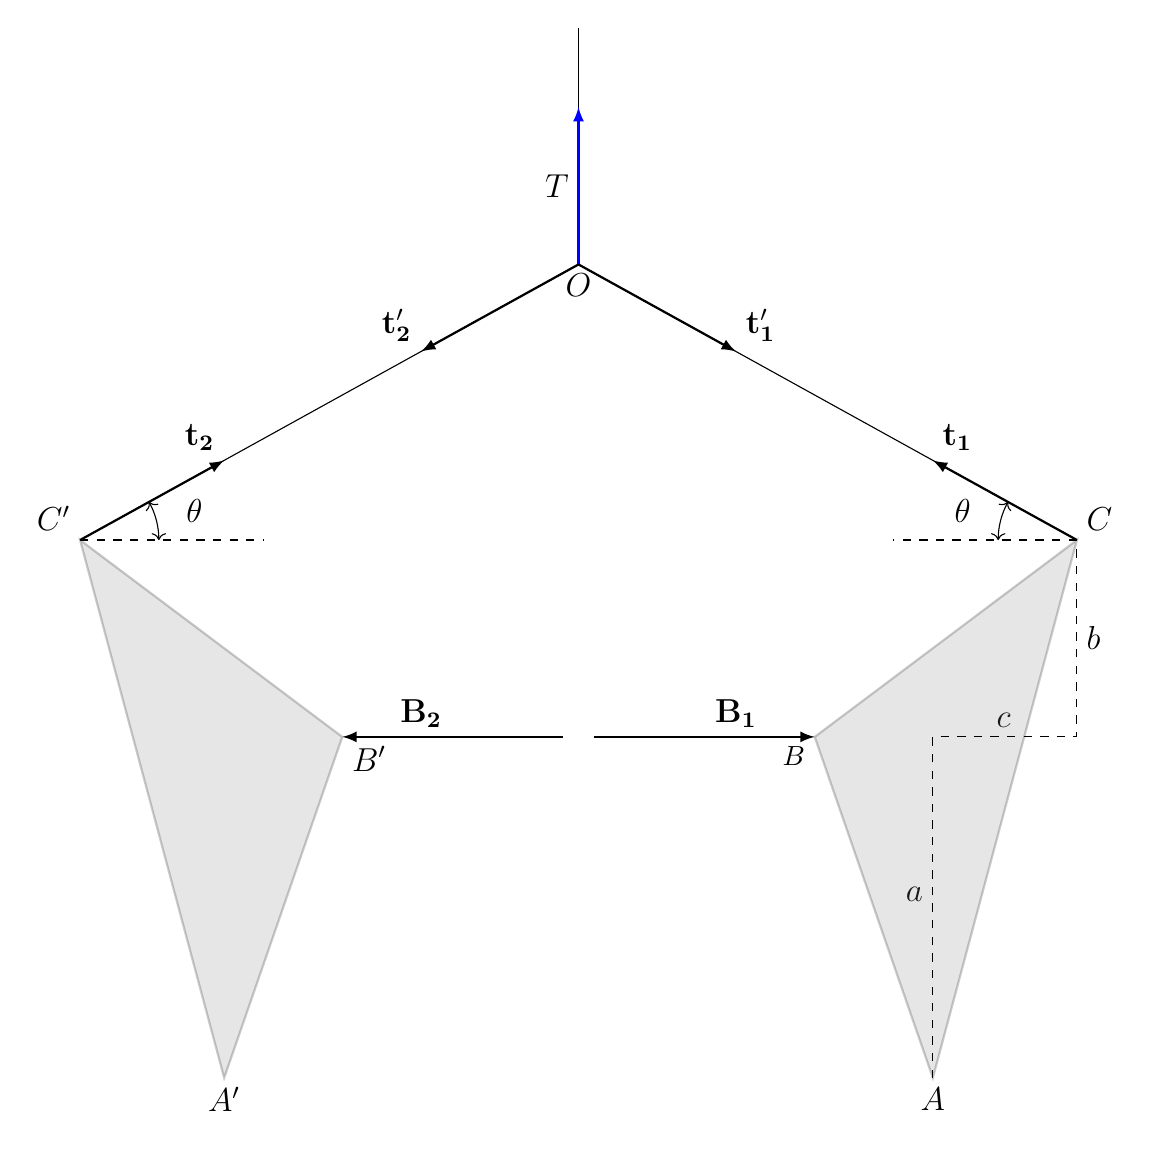
\begin{tikzpicture}		
		% B, A, C
		\coordinate[label=below left:$B$] (B) at (3,0);
		\coordinate[label=below:\large{$A$}] (A) at (4.5,-4.33);
		\coordinate[label=above right:\large{$C$}] (C) at (6.33,2.5);		
		
		% B', A', C'
		\coordinate[label=below right:\large{$B'$}] (B') at (-3,0);
		\coordinate[label=below:\large{$A'$}] (A') at (-4.5,-4.33);
		\coordinate[label=above left:\large{$C'$}] (C') at (-6.33,2.5);
		
		% O, T
		\coordinate[label=below:\large{$O$}] (O) at (0,6);
		\coordinate[label=left:\large{$T$}] (T) at (0,7);
		
		% a, b, c
		\coordinate[label=left:\large{$a$}] (a) at (4.5,-2);
		\coordinate[label=right:\large{$b$}] (b) at (6.33,1.25);
		\coordinate[label=above:\large{$c$}] (c) at (5.4,0);
		
		% B1, B2	
		\coordinate[label=above:\large{$\mathbf{B_1}$}] (B1) at (2,0);
		\coordinate[label=above:\large{$\mathbf{B_2}$}] (B2) at (-2,0);	
		
		% t1, t2		
		\coordinate[label=above right:\large{$\mathbf{t_1}$}] (t1) at (4.5,3.511);
		\coordinate[label=above left:\large{$\mathbf{t_2}$}] (t2) at (-4.5,3.511);
		
		% t1', t2'
		\coordinate[label=above right:\large{$\mathbf{t_1'}$}] (t1') at (2,4.894);
		\coordinate[label=above left:\large{$\mathbf{t_2'}$}] (t2') at (-2,4.894);
		
		\coordinate (X) at (-4,2.5);
		\coordinate (Y) at ( 4,2.5);
		
		% peças cinzas
		\draw[thick, fill=gray, opacity=0.2] (A) -- (B) -- (C) -- cycle;
		\draw[thick, fill=gray, opacity=0.2] (A') -- (B') -- (C') -- cycle;
		
		% fio
		\draw (C)--(O);
		\draw (C')--(O);
		\draw (O)--(0,9);
		
		% vetores B1, B2
		\draw[thick, -latex] (0.2,0)--(3,0);
		\draw[thick, -latex] (-0.2,0)--(-3,0);
		
		% vetor T
		\draw[thick, -latex, blue] (O)--(0,8);
		
		% vetores t1, t1'
		\draw[thick, -latex] (O)--(t1');
		\draw[thick, -latex] (C)--(t1);
		
		% vetor t2, t2'
		\draw[thick, -latex] (O)--(t2');		
		\draw[thick, -latex] (C')--(t2);
		
		% tracejado de a, b, c
		\draw[dashed] (A)--(4.5,0)--(6.33,0)--(C);
		
		% angulos
		% tracejado de auxílio
		\draw[dashed] (C')--(X);
		\draw[dashed] (C)--(Y);
		
		% thetas
		\draw pic["\large{$\theta$}", draw=black, <->, angle eccentricity=1.5, angle radius=1cm]{angle=X--C'--O};
		
		\draw pic["\large{$\theta$}", draw=black, <->, angle eccentricity=1.5, angle radius=1cm]{angle=O--C--Y};
		\end{tikzpicture}
	\end{figure}
\end{document}